\def\QRCODE{MASTER_mispa_TUT.IMG.lbp_pythonqrcode.png}
\def\QRPAGE{http://www.iptutorials.science/tree/master/MASTER_mispa/TUT.IMG.lbp/python}
\pcorrectionsection{Python correction}

The following imports are used.
\begin{python}
import numpy as np
from scipy import misc
import matplotlib.pyplot as plt
import glob
import seaborn as sn
import pandas as pd
import os
from sklearn.cluster import KMeans
\end{python}


\subsection{LBP computation}
Each pixel is given a specific 8 bits value according to a code as follows. 

\begin{python}
def LBP(I):
    B = np.zeros(np.shape(I));  
    code = np.array([[1,2,4],[8,0,16],[32,64,128]]);

    # loop over all pixels except border pixels
    for i in np.arange(1,I.shape[0]-2):
        for j in np.arange(1, I.shape[1]-2):
            w = I[i-1:i+2, j-1:j+2];
            w = w >= I[i,j];
            w = w * code;
            B[i,j] = np.sum(w);
\end{python}

Then, all values (except for border values) are summarized in the histogram.

\begin{python}
h,edges = np.histogram(B[1:-1, 1:-1], density=True, bins=256);
\end{python}

For the first image of sand, the histogram is shown in Fig.\ref{fig:lbp:python:lbpmetal1}.

\begin{figure}[H]
 \centering\caption{Illustration of the Local Binary Pattern computed on an entire image.}%
 \subfloat[Texture image.]{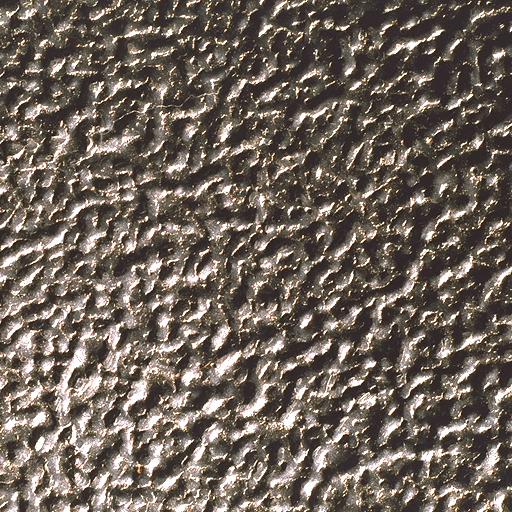
\includegraphics[width=.38\linewidth]{Metal.1.png}}\hfill
 \subfloat[LBP of texture.]{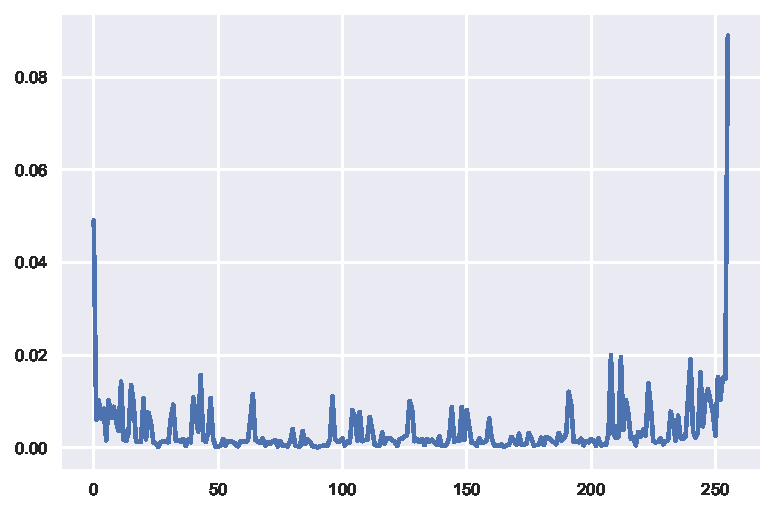
\includegraphics[width=.55\linewidth]{lbp_Metal_1.python.pdf}}%
 \label{fig:lbp:python:lbpmetal1}\vspace*{-5pt}%
\end{figure}

\subsection{Classification}
For all images of the same family, the LBP are computed and represented in the same graph. The histograms really look similar (see Fig.\ref{fig:lbp:python:lbp}). The following code is used for the ``sand'' family.

\begin{python}
classes = ['Terrain', 'Metal', 'Sand'];
names = [];
hh = [];
for c in classes:
    print(c);
    fig=plt.figure();
    for file in sorted(glob.glob('../matlab/images/'+ c + '*.bmp')):
        names.append(os.path.basename(file));
        I = imageio.imread(file);
        I = I[:,:,1];
        h, edges = LBP(I);
        plt.plot(h);
        hh.append(h);
\end{python}

 \vspace*{-5pt}%

\begin{figure}[H]
 \centering\caption{Illustration of the LBP of 4 images of each family. The histogram are almost equivalent, which shows that this descriptor can be employed to discriminate between the different families.}%
 \subfloat[Metal image example.]{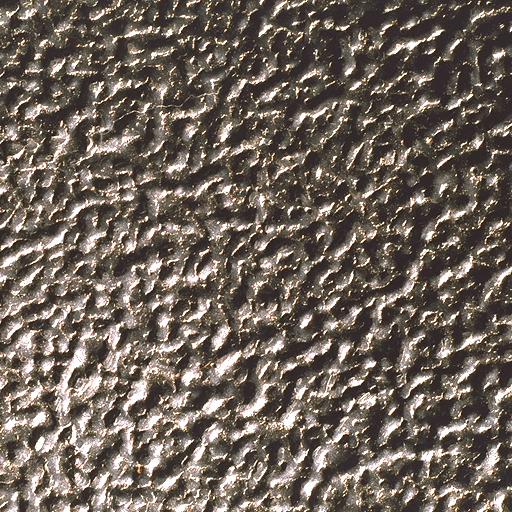
\includegraphics[width=.3\linewidth]{Metal.1.png}}\hfill
 \subfloat[Sand image example.]{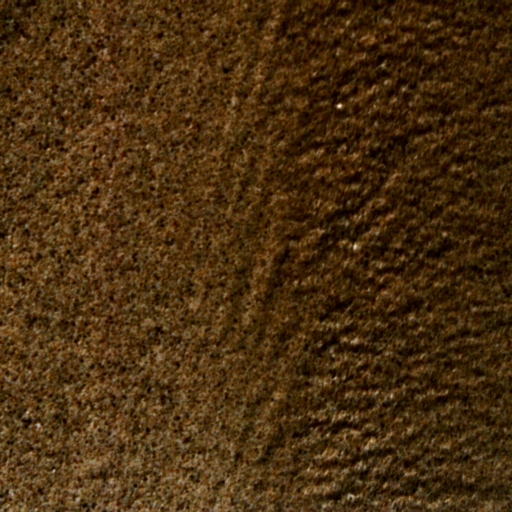
\includegraphics[width=.3\linewidth]{Sand.1.png}}\hfill
\subfloat[Terrain image example.]{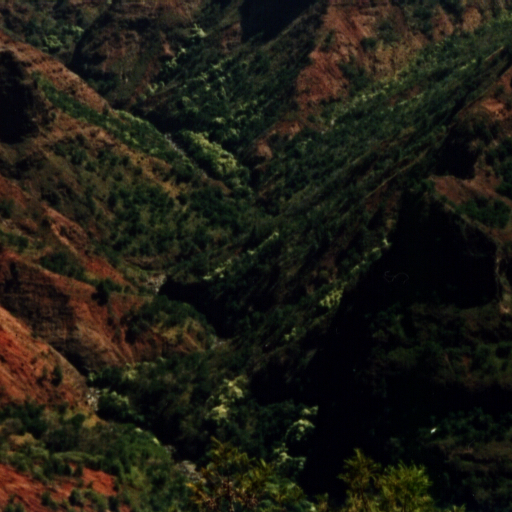
\includegraphics[width=.3\linewidth]{Terrain.1.png}}

 \subfloat[Four metal images.]{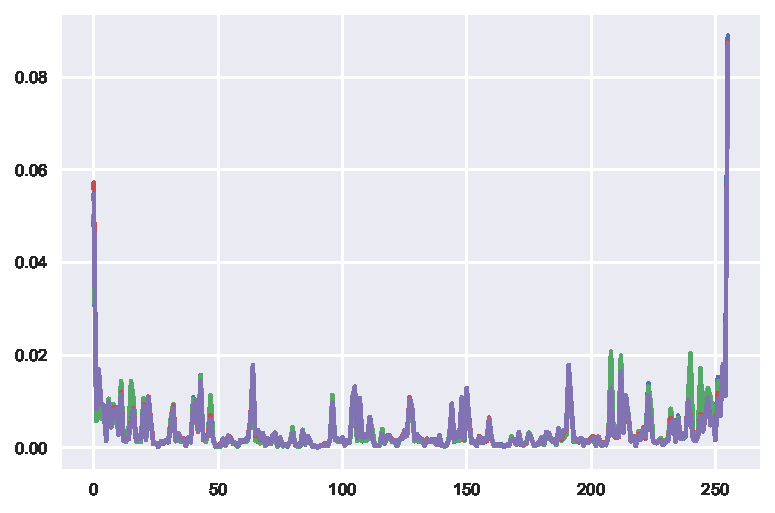
\includegraphics[width=.3\linewidth]{lbp_Metal.python.pdf}}\hfill
 \subfloat[Four sand images.]{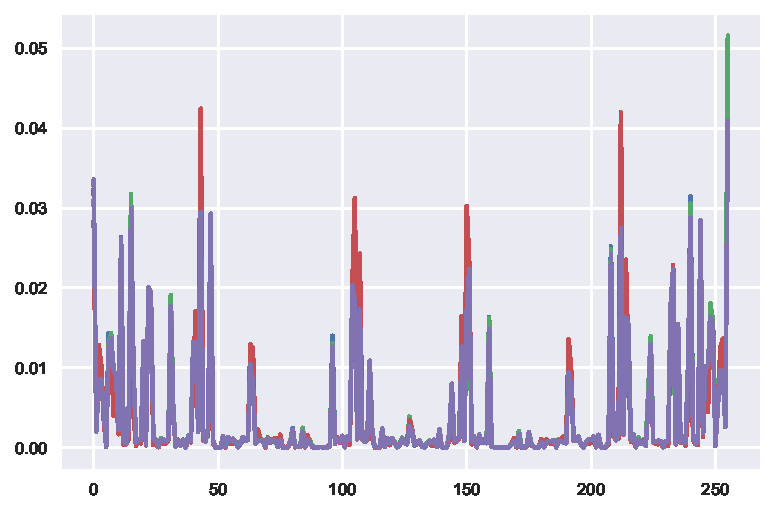
\includegraphics[width=.3\linewidth]{lbp_Sand.python.pdf}}\hfill
\subfloat[Four terrain images.]{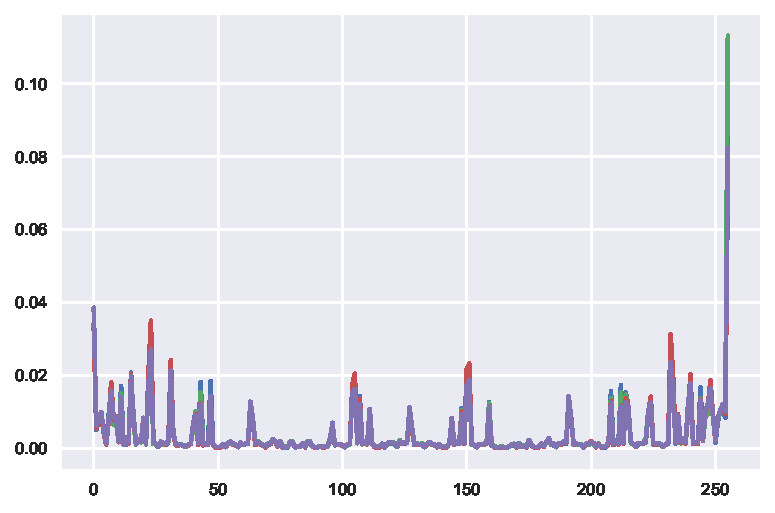
\includegraphics[width=.3\linewidth]{lbp_Terrain.python.pdf}}%
 \label{fig:lbp:python:lbp}%
 \vspace*{-10pt}%
\end{figure}
 \vspace*{-10pt}%

A distance criterion is used to compare the different histograms: the classical SAD (Sum of Absolute Differences) gives a numerical values. All pairs of distances are concatenated in a matrix, displayed as an image in Fig.\ref{fig:lbp:python:dists}.

\begin{python}
# compute distance between LBPs
n = len(hh);
dists = np.zeros((n, n))
for i in np.arange(n):
    for j in np.arange(n):
        dists[i,j] = np.sum(np.abs(hh[i]-hh[j]))
fig=plot_dists(dists, names);
\end{python}

In order to display this matrix, the module seaborn is used.
\begin{python}
def plot_dists(dists, classes, cmap=plt.cm.Blues):
    """
    Plot matrix of distances
    dists: all computed distances
    classes: labels to be used
    cmap: colormap
    returns: figure that can be used for pdf export
    """
    df_cm = pd.DataFrame(dists, index = classes, columns = classes);
    fig = plt.figure();
    sn.set(font_scale=.8)
    sn.heatmap(df_cm, annot=True, cmap = cmap, fmt='.2f');
    return fig;
\end{python}

\vspace*{-10pt}

\begin{figure}[H]
 \centering\caption{Sum of Absolute Differences between the different LBP histograms of each image. 3 families of 4 textures are represented here, terrain images are in the first part, metal images in the second and sand images in the last. Black represents 0  distance and white is 1 (highest distance, the values are normalized).}%
 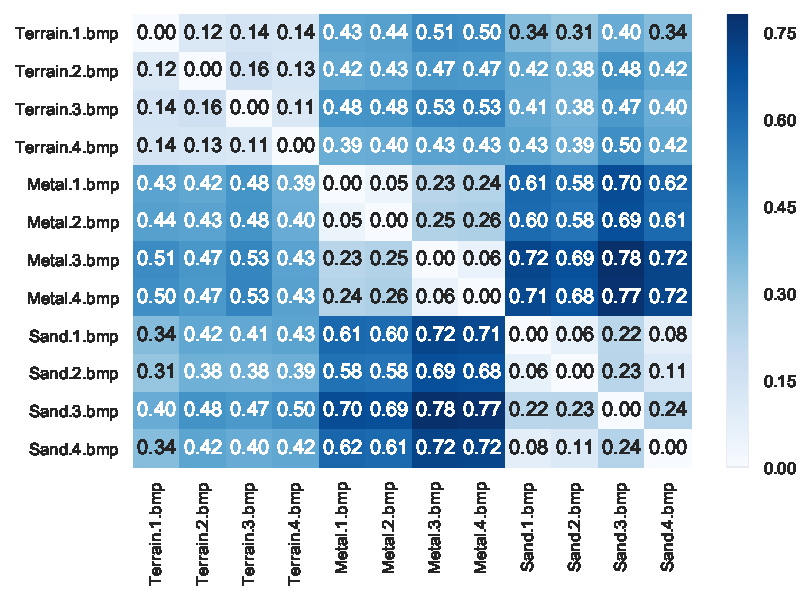
\includegraphics[width=.8\linewidth]{distances.python.pdf}%
 \label{fig:lbp:python:dists}%
\end{figure}

\vspace*{-10pt}

The kmeans algorithm uses such a distance, and we can verify that the clustering process works as expected. The result is presented in the next box.

\begin{python}
# kmeans clustering
n=3;
k_means = KMeans(init='k-means++', n_clusters=n, n_init=10)
k_means.fit(hh);
print(k_means.labels_)
\end{python}

The result show that the kmeans algorithm perfectly performs the classification.
\begin{sh}
[1 1 1 1 0 0 0 0 2 2 2 2]
\end{sh}


